\documentclass{beamer}
\usepackage{dsfont}
\usepackage{bibentry}
\usepackage{natbib}

\usepackage[utf8]{inputenc}

\newcommand{\aheader}[2]{\action<#1-|alert@#1>{#2}}
% first argument: slide number to appear from, second argument: content of header
\newcommand{\hiddencell}[2]{\action<#1->{#2}}
% first argument: slide number to appear from, second argument: content of cell

\newcommand{\EE}{\mathbb{E}}
\newcommand{\R}{\mathbb{R}}  % set of real numbers
\newcommand{\indicator}[1]{\one\left[#1 \right]} % indicator
\newcommand{\one}{\mathds{1}}
\newcommand{\ip}[2]{\left\langle #1, #2 \right\rangle} % inner product

%Information to be included in the title page:
%\title{\textbf{Bandit Multiclass Linear Classification:} \textbf{Efficient Algorithms for the Separable Case}}
%\author{Alina Beygelzimer \quad D{\'a}vid P{\'al} \quad Bal{\'a}zs Sz{\"o}r{\'e}nyi \\ Devanathan Thiruvenkatachari \quad  Chen-Yu Wei \quad  Chicheng Zhang}
%\institute{Overleaf}
%\date{ICML 2019}



\begin{document}

\frame{
\vspace{1cm}
\centering
{\color{blue} \Large \textbf{Bandit Multiclass Linear Classification:} \\
\textbf{Efficient Algorithms for the Separable Case} }
\\
\vspace{0.5cm}
\begin{minipage}{0.3\textwidth}
\centering
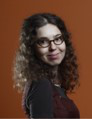
\includegraphics[height=2cm]{figures/alina.png}
\\
Alina Beygelzimer \\ (Yahoo!)
\end{minipage}
\begin{minipage}{0.3\textwidth}
\centering
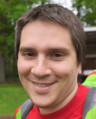
\includegraphics[height=2cm]{figures/david.png}
\\
David Pal \\ (Yahoo!)
\end{minipage}
\begin{minipage}{0.3\textwidth}
\centering
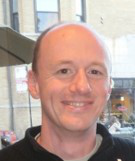
\includegraphics[height=2cm]{figures/balazs.png}
\\
Balazs Szorenyi \\ (Yahoo!)
\end{minipage}
\begin{minipage}{0.3\textwidth}
\centering
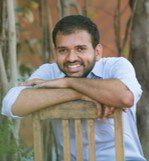
\includegraphics[height=2cm]{figures/deva.png}
\\
Devanathan
Thiruvenkatachari (NYU)
\end{minipage}
\begin{minipage}{0.3\textwidth}
\centering
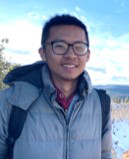
\includegraphics[height=2cm]{figures/chen-yu.png}
\\
Chen-Yu Wei \\ (USC)
\end{minipage}
\begin{minipage}{0.3\textwidth}
\centering
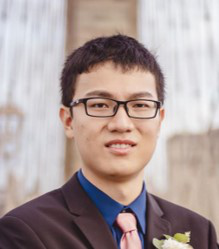
\includegraphics[height=2cm]{figures/chicheng.png}
\\
Chicheng Zhang (Microsoft)
\end{minipage}
}

\begin{frame}{Bandit multiclass classification}

\begin{minipage}{0.6\textwidth}
For $t=1,2,\dots,T$:
\begin{enumerate}
\item<2-> Example $(x_t, y_t)$ is chosen, where \\
\qquad \action<3->{$x_t \in \R^d$ is the {\color{red}feature (shown to the learner)},} \\
\qquad \action<4->{$y_t \in [K]$ is the {\color{blue}label (hidden)}.}\\
\item<5-> Predict class label $\widehat y_t \in [K]$.\\
\item<6-> Observe feedback $z_t = \indicator{\widehat y_t \neq y_t} \in \{0,1\}$.
\end{enumerate}
\end{minipage}
\hspace{0.3cm}
\begin{minipage}{0.35\textwidth}

\begin{columns}
\begin{column}{0.35\textwidth}
\vspace{-1.5cm}
\action<4->{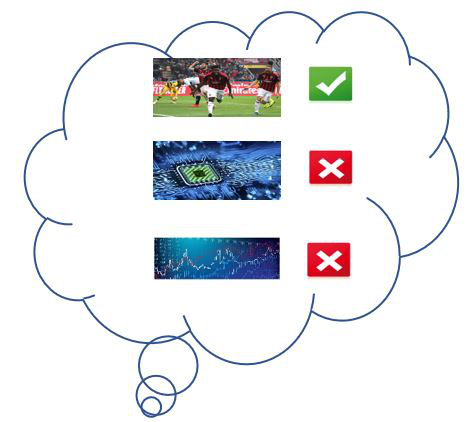
\includegraphics[width=1.8\linewidth]{figures/label.png}}
\\
\action<2->{
\includegraphics[width=\linewidth]{figures/user.png}}
\end{column}
\begin{column}{0.3\textwidth}
\\
\centering
\action<3->{
\includegraphics[width=0.5\linewidth]{figures/info.png}
\\
\vspace{-0.3cm}
$\xrightarrow{\hspace*{\linewidth}}$}
\\
\action<5->{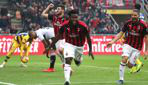
\includegraphics[width=0.5\linewidth]{figures/action.png}
\\
\vspace{-0.3cm}
$\xleftarrow{\hspace*{\linewidth}}$}
\\
\action<6->{
\includegraphics[width=0.3\linewidth]{figures/feedback.png}
\\
\vspace{-0.3cm}
$\xrightarrow{\hspace*{\linewidth}}$
}
\end{column}
\begin{column}{0.35\textwidth}
\vspace{0.3cm}
\action<1->{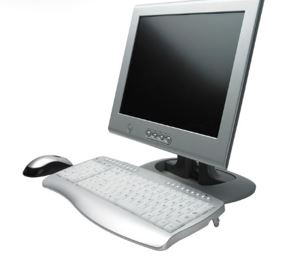
\includegraphics[width=\linewidth]{figures/learner.png}}
\end{column}
\end{columns}
\end{minipage}

\action<7->{
\vspace{1cm}
Goal: minimize the total number of mistakes
$\sum_{t=1}^T z_t$.}
\end{frame}

\begin{frame}{Challenge: efficient algorithms in the separable setting}

\begin{definition}
A dataset is called $\gamma$-linearly separable
if there exists $w_1, \ldots, w_K$ such that
\begin{align*}
\ip{w_{y}}{x} \ge \ip{w_{y'}}{x} + \gamma, \qquad \forall y' \neq y,
\end{align*}
for all $(x,y)$ in the dataset. (with the constraint $\sum_{i=1}^K \|w_i\|^2\leq 1$)
\end{definition}

\action<2->{
\centering
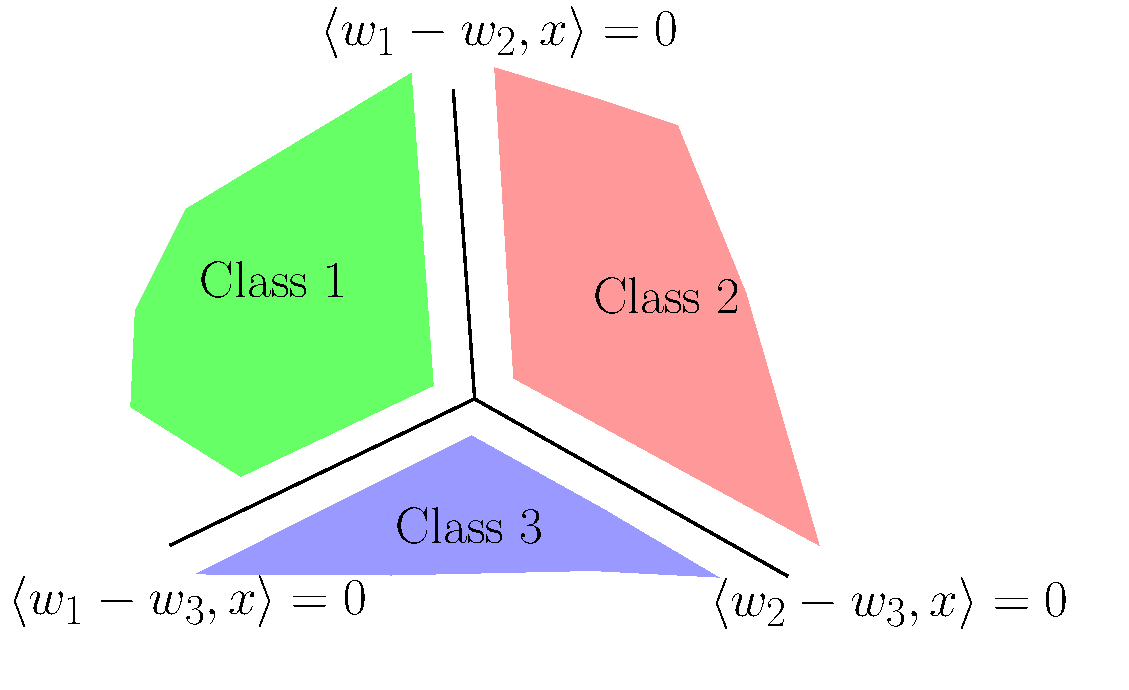
\includegraphics[width=0.6\linewidth]{figures/weak_sep.pdf}
}


\end{frame}


\begin{frame}{Related work}

\bgroup
\def\arraystretch{2}%  1 is the default, change whatever you need
\begin{tabular}{|l|l|l|}
\hline
\hiddencell{1}{Algorithm} & \hiddencell{1}{Mistake Bound} & \hiddencell{1}{Efficient?} \\
\hline
\hiddencell{2}{Minimax algorithm~\cite{Daniely-Helbertal-2013}} &     \hiddencell{2}{$O(K/\gamma^2)$} &
\hiddencell{2}{No} \\
\hline
\hiddencell{3}{Banditron~\cite{Kakade-Shalev-Shwartz-Tewari-2008} \footnote{See also~\citep[][..]{Hazan-Kale-2011, Beygelzimer-Orabona-Zhang-2017, Foster-Kale-Luo-Mohri-Sridharan-2018} that have similar guarantees}} &     \hiddencell{3}{$O(\sqrt{TK/\gamma^2 })$}  &  \hiddencell{3}{Yes} \\
\hline
\hiddencell{4}{{\color{red}This work}} &     \hiddencell{4}{$2^{\widetilde{O}(\min(K \log^2
(1/\gamma), \sqrt{1/\gamma} \log K))}$} &     \hiddencell{4}{Yes}\\
\hline
\end{tabular}
\egroup
\ \\
\ \\
\ \\
\action<5->{\textbf{Contribution}: first efficient algorithm that breaks the $\sqrt{T}$ barrier}

\end{frame}


\begin{frame}{Algorithm}
(One-versus-rest approach)\\
\ \\
\hspace*{-30pt}
\begin{minipage}{0.48\linewidth}
\action<2->{
    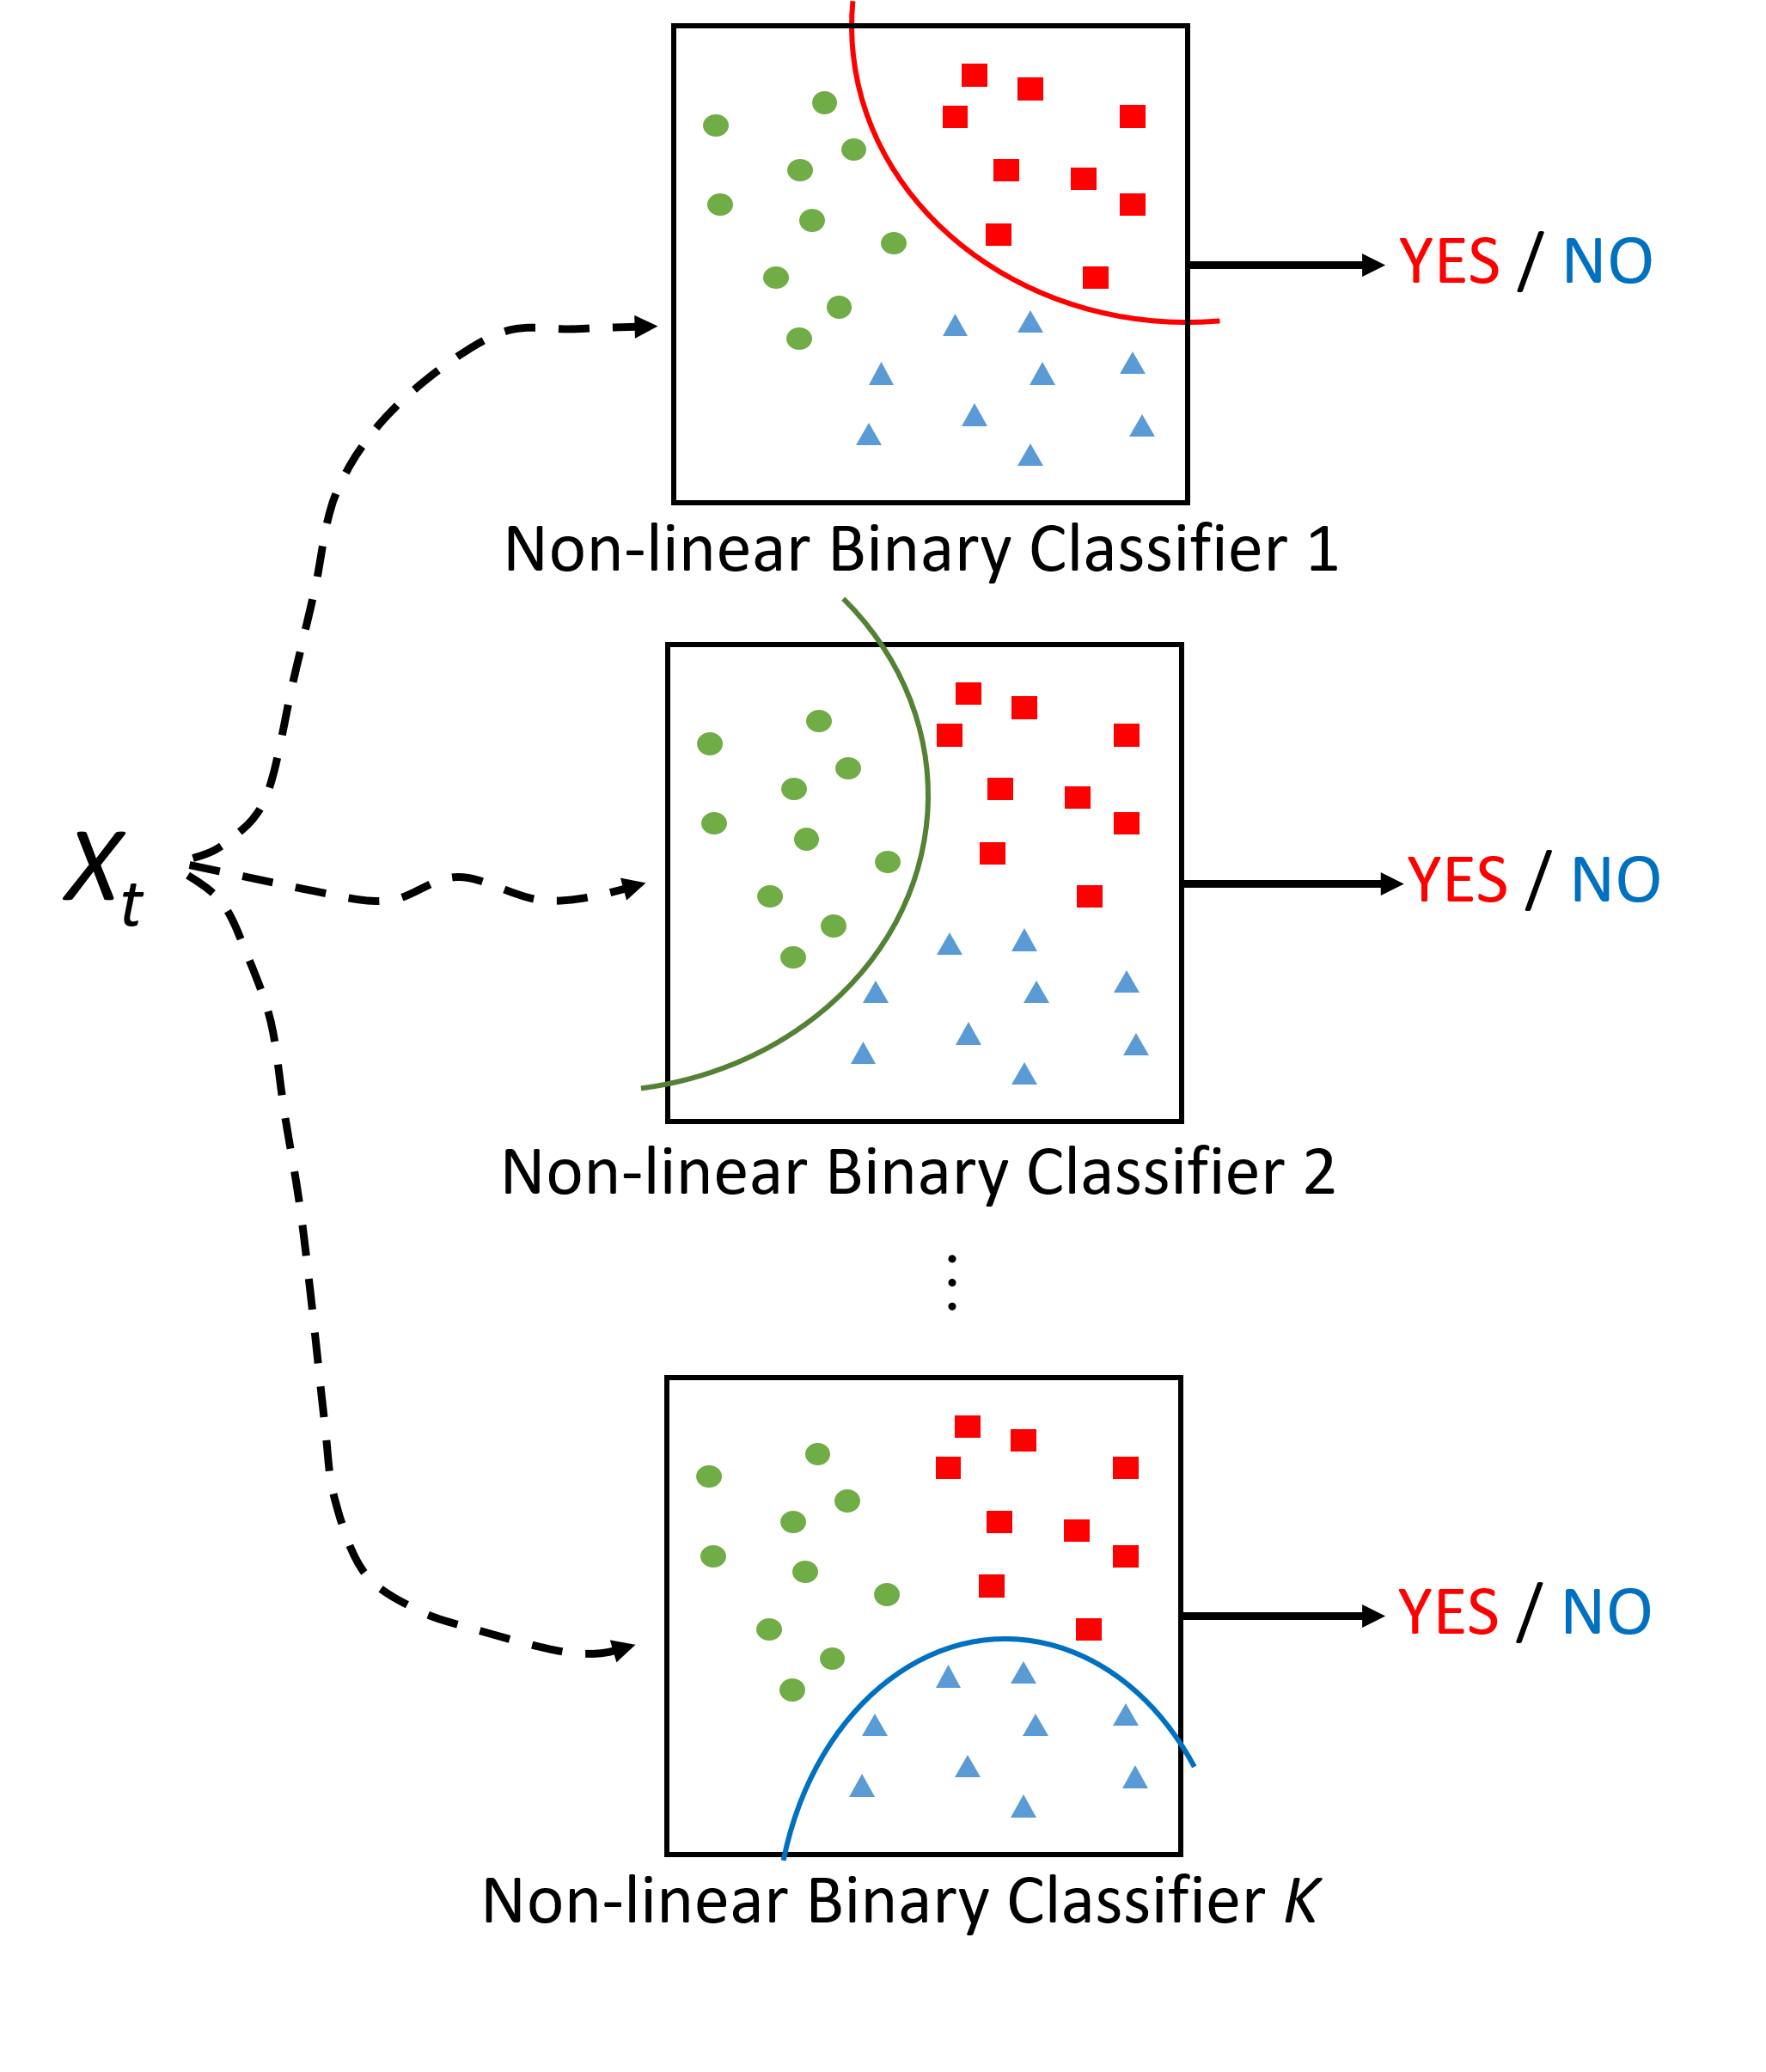
\includegraphics[ width=\textwidth]{figures/algorithm.png}
}
\end{minipage}
\hfill
\begin{minipage}{0.58\linewidth}
\action<3->{
    If $\geq 1$ of them respond {\color{red} YES}:\\
    $\widehat{y}_t\leftarrow$ any one of those {\color{red}YES} labels\\
    \ \\
    If all of them respond {\color{blue} NO}:\\
    $\widehat{y}_t\leftarrow$ uniform from $\{1,\ldots, K\}$\\
}
\action<4->{
    \ \\
    \ \\
    \fbox{$\EE[\#\text{mistakes(alg)}] \leq K\sum_{i}\#\text{mistakes($i$)}$}
}
\end{minipage}

\end{frame}

\begin{frame}{Algorithm}
    %\begin{center}
    %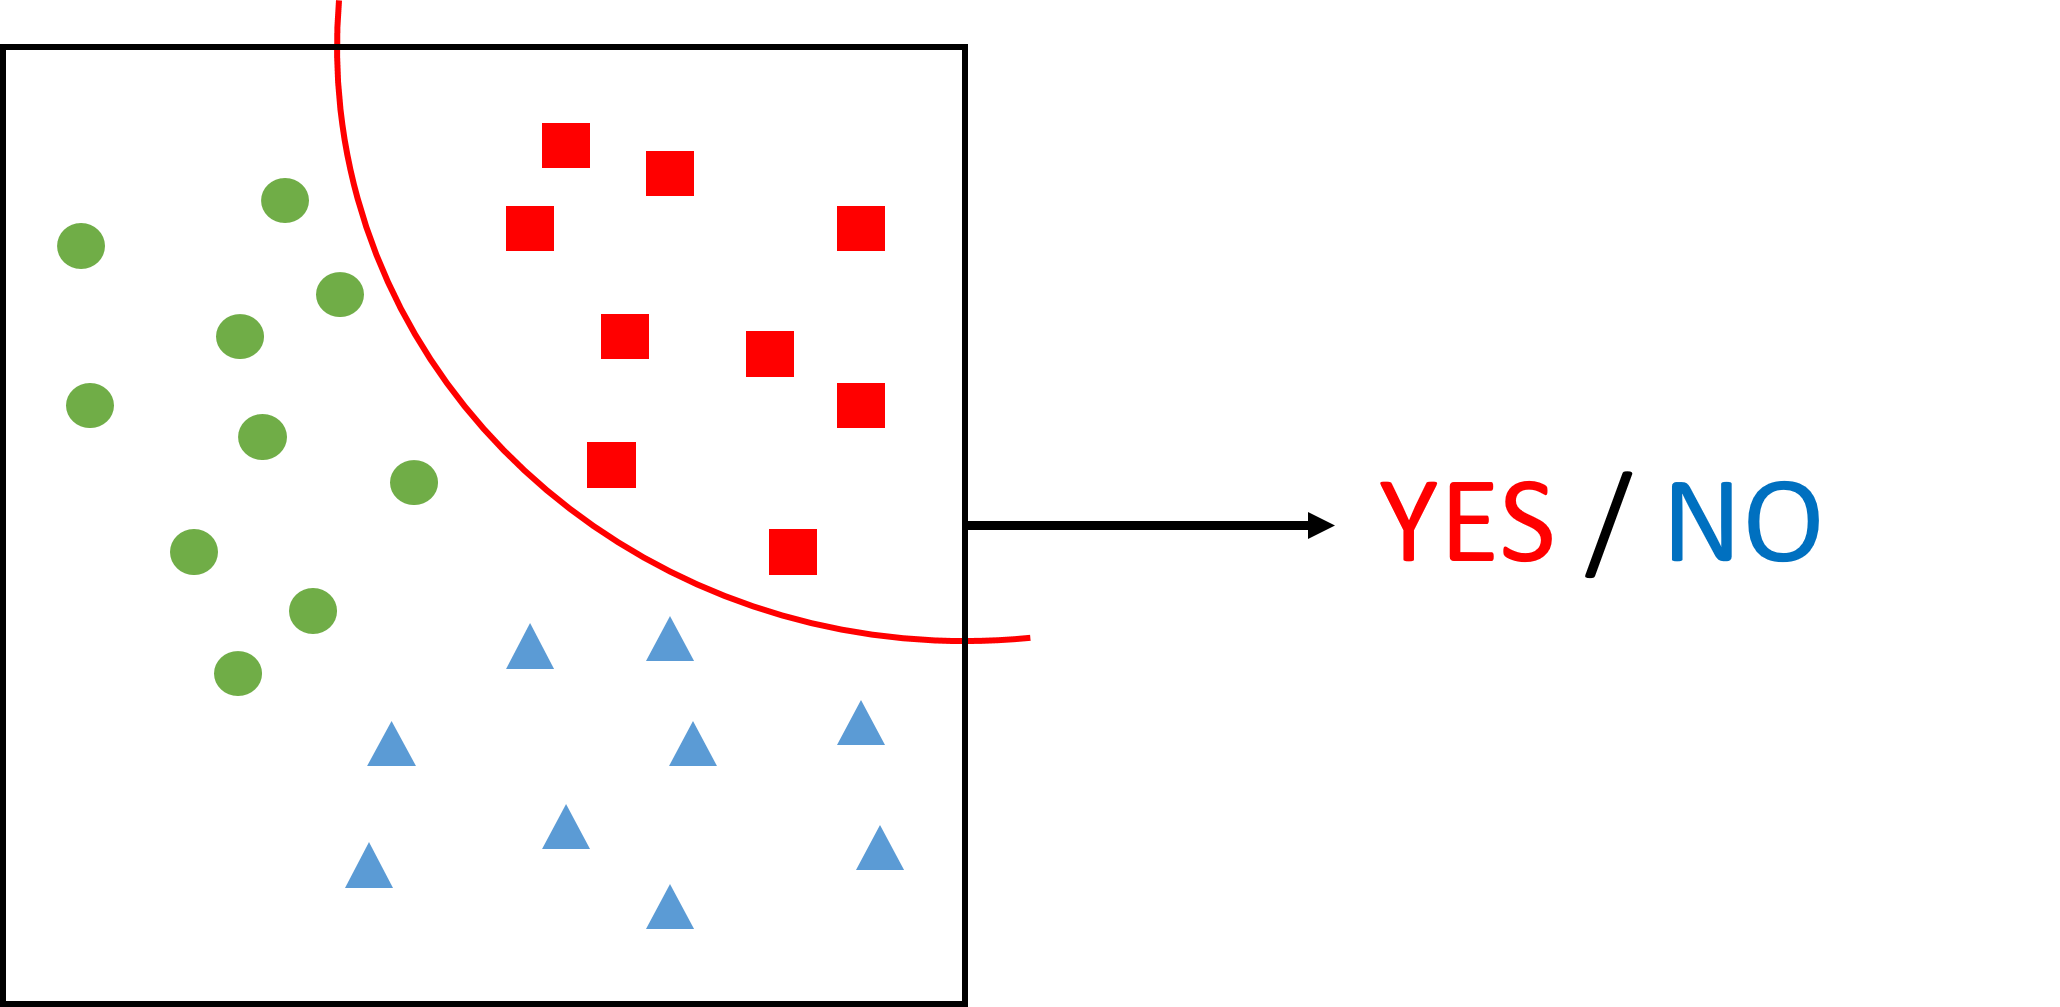
\includegraphics[width=0.5\textwidth]{figures/kernel_perceptron.png}
    %\end{center}
    \begin{itemize}
        \item<1-> Each non-linear binary classifier learns the support of class $i$, which lies in an intersection of $K-1$ halfspaces with a margin~\citep{Klivans-Servedio-2004}.\\
        \centering
        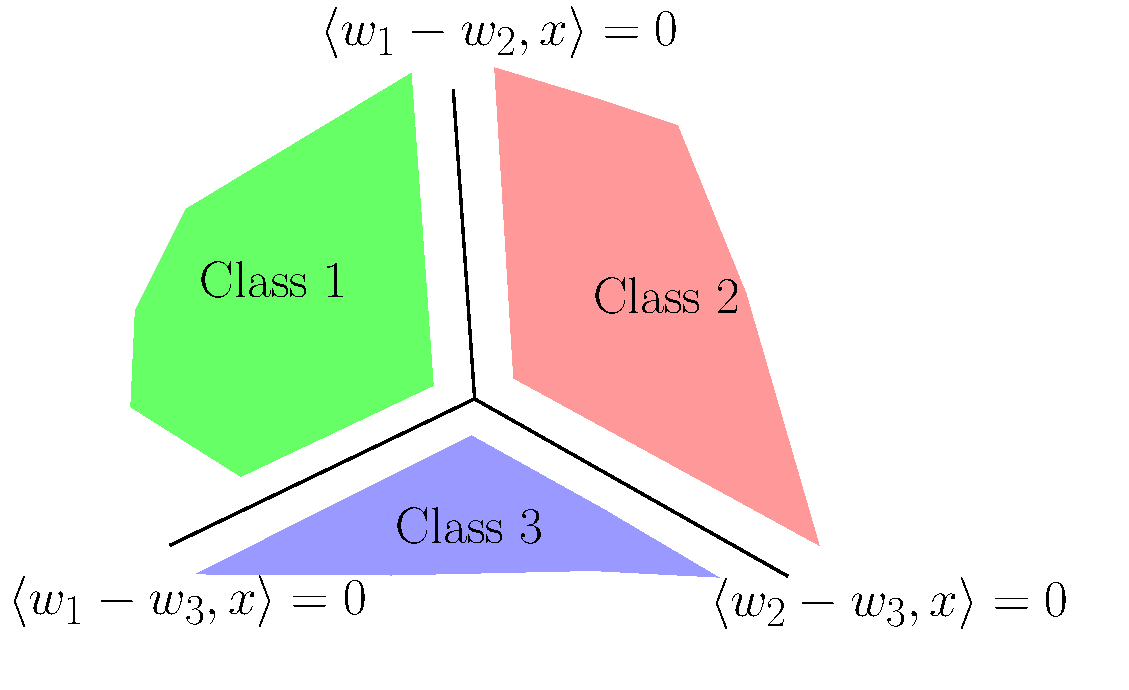
\includegraphics[width=0.6\linewidth]{figures/weak_sep.pdf}
        \item<2-> Choice: \textbf{kernel Perceptron} with \textbf{rational kernel}~\cite{Shalev-Shwartz-Shamir-Sridharan-2011}:
        \begin{align*}
            K(x, x') = \frac{1}{1-\frac{1}{2}\langle x, x'\rangle}.
        \end{align*}
        \item<3-> {\color{red}\fbox{Thu. Poster\#158}}


    \end{itemize}
\end{frame}


%\begin{frame}{Side results}
%    \begin{itemize}
%        \item<1-> Slightly improving \citep{Klivans-Servedio-2004}'s result on learning intersections of halfspaces.
%        \item<2-> Two hardness results that indicate this problem cannot be solved by a certain types of algorithms.
%         \begin{itemize}
%         \item<3->  Unfortunately, most previous efficient bandit classification or contextual bandit algorithms are of these types.{\color{green}(CZ: I am not sure if we should mention this, for example Banditron is technically not an ignorant algorithm.. And what is the second hardness result - is it about the intersection of two halfspaces problem?)}
%         \end{itemize}
%    \end{itemize}
%\end{frame}

\bibliographystyle{alpha} % Plain referencing style
\nobibliography{biblio} % Use the example bibliography file sample.bib

\end{document}
